\chapter{Bilan de planification}

\paragraph{}
Conformément au rapport de conception, nous avons construit le projet sur deux itérations. La première réduisait l'interface au maximum tout en répondant au cahier des charges. Cette interface permettait donc d'ouvrir un document de travail, et de valider ou invalider les transcriptions. La première itération a été rendue avec un mois de retard, en accord avec l'encadrant de projet. Le but est ici d'en expliquer les raisons. Nous nous intéresserons d'abord aux problèmes rencontrés, à la quantification des impacts de ces problèmes, et aux connaissances acquises pour les projets futurs.

\section{Problèmes rencontrés}

\paragraph{}
Lors de la phase de réalisation du projet au second semestre, nous avons été confrontés à plusieurs problèmes, listés comme risques dans le rapport de planification pour la plupart. Nous allons détailler les trois problèmes principaux.

\paragraph{}
Le premier élément qui nous a concernés faisait partie de la liste des risques dans le rapport de planification. Il s'agit de la surcharge de travail avec les cours. Pour éviter ce problème, nous avions prévu de prendre de l'avance au semestre précédent, qui était cependant très chargé. Nous avons réussi à dégager des heures de travail, qui ont servi à installer et mettre en place les différentes technologies nécessaires au projet. Cette phase d'installation a pris beaucoup plus de temps que prévu, et nous nous sommes retrouvés avec une installation partiellement effectuée en début de S8, mais très peu de code utile au projet préparé à l'avance. Cette solution d'anticipation n'a donc pas fonctionné, et nous avons pris du retard. Un autre facteur était la quantité d'éléments présents dans le cahier des charges. En effet, nous avons vu trop grand au départ, en sous-estimant le temps nécessaire pour développer le logiciel, ce qui semble toutefois être une erreur récurrente chaque année en 4INFO.

\paragraph{}
Un second élément inattendu était une mauvaise pratique logicielle. En d'autres termes, dans le souci de bien faire, et de par nos habitudes en cours, nous avons souhaité dans un premier temps réaliser l'intégralité du projet en un seul bloc, tout le code étant écrit en Scala ou Java. Ceci s'est révélé être une solution beaucoup moins efficace que celle que nous avons finalement mise en place, qui consiste à utiliser des scripts externes pour nous aider au besoin. Par exemple, pour traiter les documents de la base Maurdor, nous avons écrit un script Python qui parcourt un dossier et qui découpe les pages des documents ainsi que leurs vérités terrain, pour obtenir un couple image - vérité terrain par page de chaque document. La découpe d'images est également réalisée avec un script externe. La bibliothèque graphique est toujours OpenCV comme prévu initialement, mais cette bibliothèque a un très mauvais support de Java, et est beaucoup plus mature en C++ et en Python. Il était donc plus raisonnable d'utiliser la bibliothèque dans un script Python, et de l'appeler depuis notre application en Scala, d'autant plus que Scala propose une manière concise et élégante d'appeler des commandes externes, via un opérateur dédié à cette tâche.

\paragraph{}
Le dernier élément auquel nous avons été confrontés est l'absence d'un des membres du groupe, Valentin. En effet, il avait déjà été beaucoup absent au premier semestre pour raison personnelle, et n'avait pu nous aider que sur le rapport de pré-étude du projet. Nous pensions pouvoir le réintégrer à l'équipe au second semestre, en lui proposant des tâches qui pourraient nous aider sans pour autant prendre trop de risques, c'est-à-dire que nous lui avons confié des tâches non critiques. Il n'a malheureusement pas pu les effectuer, et a quitté l'équipe du projet car il souhaite quitter l'INSA et se réorienter. Ce sont des choses qui arrivent, mais ayant prévu des heures pour Valentin à la fois dans la planification et en réunion avec l'encadrant au second semestre, nous avons réparti son travail entre les membres du groupe, et avons effectué l'intégralité de la partie technique du projet à quatre, ce qui a accentué l'effet du premier élément mentionné, à savoir la surcharge de travail. Au total, un mois de retard a été comptabilisé, et accepté par l'encadrant au vu de ces circonstances particulières.

\section{Quantification des impacts}

\paragraph{}
Pour garder une trace du temps passé sur chaque partie du projet, nous avons tenu une table des temps pour chaque personne sur un tableur partagé entre nous. Cet outil nous permet de dresser le tableau comparatif final ci-dessous.

\begin{center}
    \begin{tabular}{ | l | l | l | }
        \hline
        \multicolumn{3}{ | c | }{ \textbf{Comparaison des temps prévus et réels} } \\
        \hline
        \textbf{Sous-partie du projet} & \textbf{Temps prévu} & \textbf{Temps réel} \\
        \hline
        Préparation des données & 77h & 45h \\
        \hline
        Stockage des données & 10h & 16h \\
        \hline
        Interface avec le reconnaisseur & 40h & 17h \\
        \hline
        Interface Homme-Machine & 85h & 70h \\
        \hline
        Rapports et soutenances & 63h & 75h \\
        \hline
        Général & 16h & $\sim$ 5h \\
        \hline
        API REST et contrôleur & 0h & 56h \\
        \hline
        Installation et prise en main des technologies & 0h & 18h \\
        \hline
        \textbf{Total} & \textbf{291h} & \textbf{$\sim$ 302h} \\
        \hline
    \end{tabular}
\end{center}

\paragraph{}
Au vu du rapport de planification et du temps de travail effectué, on peut voir que la différence entre les heures de travail théoriques sur le projet et les heures réelles est faible dans le total, mais conséquente si l'on regarde partie par partie, pour plusieurs raisons. La première raison est que nous avons prévu des marges et évalué toutes les durées à la hausse par sécurité, ce qui augmente le nombre d'heures à passer sur le projet pour être certain de le terminer à temps. Cela explique la différence d'heures pour les parties de préparation des données, interface avec le reconnaisseur, IHM. La deuxième raison est que nous avons passé du temps sur des parties non prévues dans la planification initiale. Par exemple, la définition, l'implémentation, et le test de l'API REST ont pris un nombre d'heures conséquent, qui n'était pas prévu dans le rapport de planification. Il en est de même pour l'installation et la prise en main des technologies. Nos disponibilités par semaine ont donc été une bonne estimation, mais la répartition de ces heures l'était moins, comme nous pouvons le constater dans la Figure X.

\paragraph{}
En termes de dates, le projet avait été planifié sur deux itérations, la première étant pour le 27 février et la seconde pour le 26 avril. La première itération a été rendue le 5 avril, et la seconde en fin d'année, le 9 mai. Un mois de retard a donc été comptabilisé pour la première itération, qui était peu solide et allégée par rapport aux éléments prévus. Il était possible de visualiser des exemples déjà ajoutés dans la base de données, ainsi que de créer des nouveaux projets, mais tous les éléments de ces projets devaient être ajoutés à la base de données manuellement, ce qui en fait une version peu utilisable. La seconde itération a rattrapé la moitié de ce retard, du fait d'une simplification du cahier des charges, et d'une mise en oeuvre plus expérimentée au niveau technique. Les fonctionnalités essentielles pour générer des ensembles d'entraînement pour les reconnaisseurs d'écriture manuscrite sont réunies, comme nous pouvons le constater dans une annexe précédente de ce rapport. D'autres fonctionnalités prévues ont été annulées. Ayant un nombre d'heures global cohérent avec la théorie, on a donc ici la confirmation que nous avons sous-estimé le nombre d'heures de travail sur chaque partie.

\begin{mdframed}[frametitle={Figure 1 : Répartitions théorique et réelle des heures du projet}, innerbottommargin=10]
\begin{center}
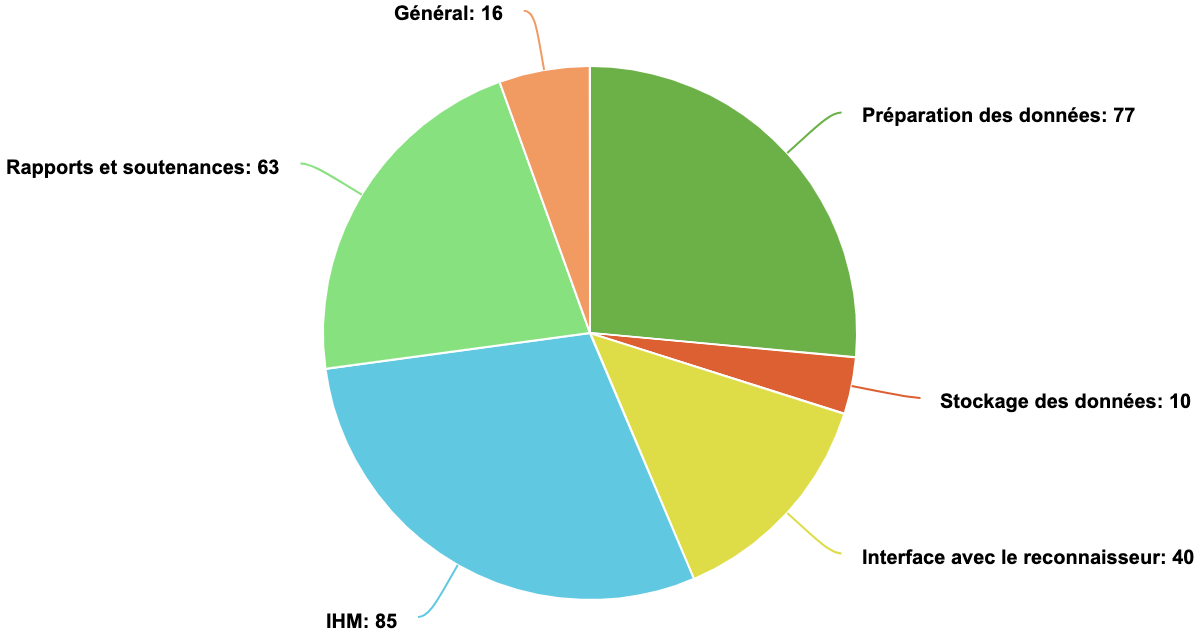
\includegraphics[scale=0.6]{assets/repartition1.png}
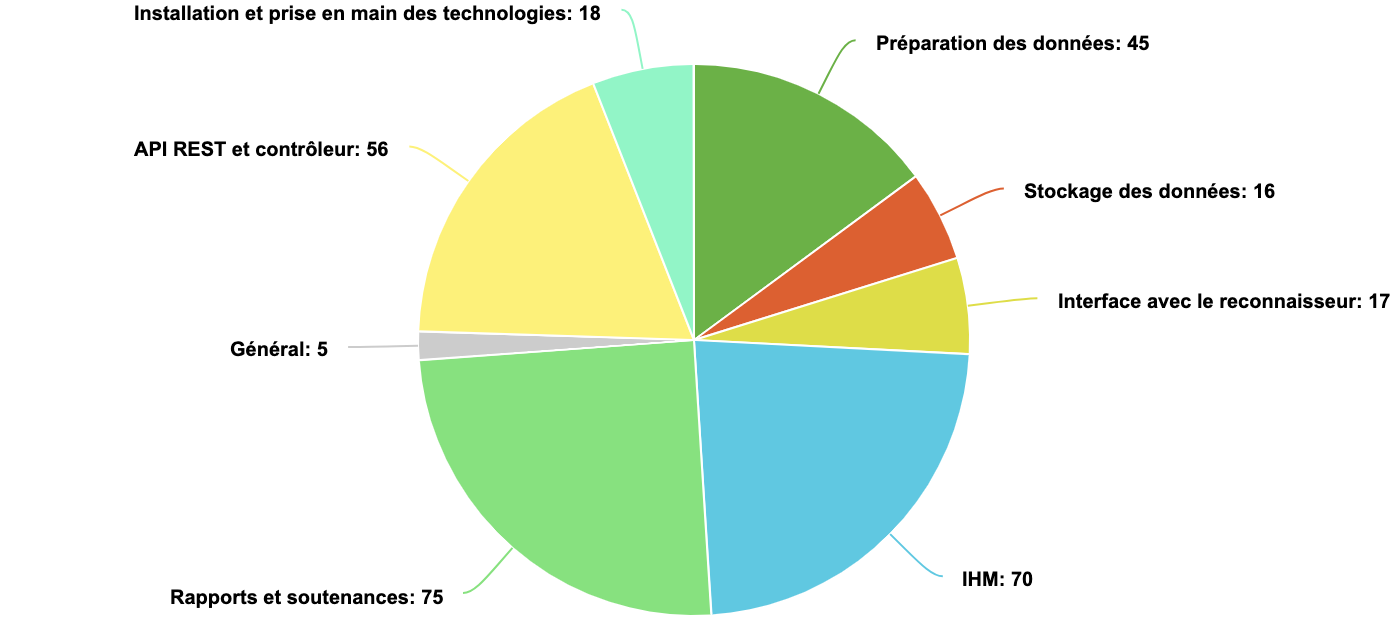
\includegraphics[scale=0.6]{assets/repartition2.png}
\end{center}
\end{mdframed}

\section{Conclusions et connaissances acquises pour les projets futurs}

\paragraph{}
Pour résumer, on peut dire que le retard est lié à trois éléments : une mauvaise estimation du temps nécessaire sur les différentes tâches, des mauvais choix logiciels au début du projet, et le départ d'un membre de l'équipe pour la phase de développement.

\paragraph{}
Le premier point nous a apporté de l'expérience en gestion pour les projets futurs. En effet, nous avons à présent vécu un projet dans lequel nous avons sous-estimé le temps pris par les différentes tâches de la phase de développement. En d'autres termes, nous pouvons dire que nous avons obtenu la preuve empirique que le développement ne peut pas se résumer à l'écriture du code. L'installation et la configuration des différents logiciels et technologies utilisés peut prendre un temps non négligeable, ce à quoi nous n'avons pas fait assez attention. Partir d'une solution simple, puis ajouter peu à peu des améliorations logicielles, c'est-à-dire voir le cahier des charges comme un objet itératif, semble également être une méthode à privilégier.

\paragraph{}
Le second point nous a apporté de l'expérience quant à lui sur la phase de développement. Nous avons bien compris le fait qu'une application en bloc unique entièrement écrite dans le même langage n'est pas toujours la meilleure solution. Dans un tel projet destiné à des chercheurs, ajouter un langage (qui plus est, répandu) dans les dépendances du logiciel n'est pas une contrainte, et les développeurs ne doivent pas hésiter à scripter certaines tâches, surtout lorsque cette solution est beaucoup plus simple que de s'entêter à vouloir intégrer ces tâches à l'intérieur du logiciel principal. Les langages de script, comme leur nom l'indique, sont faits pour répondre à ce genre de besoins, en permettant de développer des scripts annexes qui viennent appuyer efficacement un plus gros projet.

\paragraph{}
Enfin, le dernier point a permis de montrer que malgré toute planification préalable, un projet peut toujours avoir des imprévus d'ordre plus ou moins important. Dans notre cas, développer la partie technique d'un projet à quatre et sans reprise de code a été un réel défi, et nous avons fait au mieux lors de ce semestre pour livrer un logiciel fonctionnel en conservant un maximum d'éléments du cahier des charges d'origine.